%------------------------------%
\chapter[Enhancing Social Experience via Context Sharing]{Enhancing Social Experience in Normative Agents via Context Sharing}
\label{chap:poros}
%------------------------------%

This chapter describes \frameworkB, our approach for building
personal agents that carry out enriched interactions where deviating
agents share selected elements of their contexts, and others
respond appropriately, and its empirical evaluation via 
simulation experiments. It is based on a paper ``Robust Norm 
Emergence by Revealing and Reasoning about Context: Socially 
Intelligent Agents for Enhancing Privacy'' that appears in 
\emph{ Proceedings of the 27th International Joint Conference 
on Artificial Intelligence (IJCAI)}.

\section{Introduction}
\label{sec:Poros-intro}

Social \emph{norms} provide a robust means to regulate interactions in 
human society. Our everyday actions tend to \emph{comply} with social norms. For example, \fsl{ignoring a phone call during a 
meeting} and \fsl{remaining silent in a public library} are expected 
behaviors that accord with social norms. However,  we often \emph{deviate} from the applicable social norms, for 
instance, when \fsl{stepping out of a meeting to answer a phone call}.

The ability to deviate from norms is crucial for autonomy. We 
may \emph{sanction} each other based on how we
are interacting. In particular, negative sanctions in response to
deviations are a means for establishing norms \citep{Andrighetto-2013-PunishVoice}. 
For example, when a meeting attendee's phone rings, a \fsl{scowl} on other attendees'
faces hints at a norm of \fsl{keeping one's phone silent
during meetings}.

Existing approaches for norms provide simplified interactions: a deviation or not, followed by a sanction or not. But real-life interactions are more complex. Whether a deviation leads to a positive or negative sanction depends on 
how others perceive its \emph{context} or circumstances of occurrence. 
When we deviate from a norm, we may offer an apology, describing the 
context. One, revealing context may soften a deviation and help avert 
negative sanctions. Suppose, upon receiving a call during a meeting, 
Alice says that the call was from her sick father. As a result, the meeting attendees may excuse Alice for taking 
the call. A deviation may result in a positive sanction. For instance, 
a physician who reveals a patient's private data to save the patient's life 
would receive a positive sanction despite violating a norm. 
Even in the phone call setting, a positive sanction may ensue for deviating from a norm. For
example, a user who hesitantly takes a call from his nine-month
pregnant wife during a lab meeting would generally receive positive
comments from coworkers.
%
Two, context helps refine the relevant norms. For example, Alice's 
revelation may help refine the norm from \fsl{ignoring a phone call 
during a meeting} to \fsl{ignoring a phone call during a meeting, unless 
the call is urgent}. In essence, deviation context and any ensuing 
sanction help characterize the boundaries of a norm in play.

Accordingly, we propose \frameworkB, an approach for building agents that carry out enriched interactions where deviating agents share selected elements of their contexts, and others respond appropriately. A socially intelligent personal agent (SIPA) is an agent who acts in accordance with (but may deviate from) social norms \citep{Ajmeri-AAMAS17-Arnor}.  
%
We imagine an artificial agent society in which SIPAs of three main types act and interact on behalf of (human) users, as a basis for empirically investigating the emergence and quality of norms. 

This research applies in developing privacy-supporting SIPAs. Norms provide a basis for understanding privacy \citep{Nissenbaum-11:online}. Regulations about information disclosure, as in healthcare, are context-dependent norms \citep{Ajmeri-IJCAI16-Coco}, as are social practices. Privacy involves control over when and what information to disclose \citep{westin1967privacy}. In some construals, actions that intrude upon one's solitude or bring disapprobation are privacy violations. In essence, all privacy-relevant interactions are modulated by norms.  Therefore, social intelligence in making decisions cognizant of norms while preserving social cohesion is crucial.

%\paragraph{Contribution}
%
Our main contribution is to study two research questions in light of a specific decision by a SIPA, namely, whether to reveal its context to others when it deviates from a norm:

\begin{description}
\item[Q$_1$ Norm:] Does revealing context and reasoning about revealed context promote emergence of robust social norms? 
\item[Q$_2$ Goal:] Does acting in accordance to such robust norms result in an improved goal satisfaction?
\end{description}

Our results show that (1) norms that emerge in \frameworkB are robust, implying improved social cohesion and (2) SIPAs yield higher goal satisfaction to their users when acting in \frameworkB than when acting in a conventional setting (just sanctions). 

\section{Related Work}
\label{sec:Poros-related-work}

Research on normative systems has addressed the problems of conflict, 
compliance, and emergence of norms. We sample some of the literature from the following themes.

%\paragraph{Social Norms and Multiagent Systems}
\emph{Social norms} regulate agent interactions by characterizing
what behavior one agent may legitimately expect from another in a particular 
setting \citep{Kafali-IS16-Revani,Singh-2013-Norms}. 
%
We adopt Singh's \shortcite{Singh-2013-Norms} computational representation 
of social norms. A norm is directed from a subject (stakeholder) to an 
object (stakeholder), and is constructed
as a conditional relationship involving an antecedent (which brings the
norm into force) and a consequent (which brings the norm to satisfaction
or violation). 
Ajmeri {\etal} \shortcite{Ajmeri-AAMAS17-Arnor} 
introduce Arnor, a method to model social intelligence in personal agents. 
They argue that personal agents who understand 
the intricacies of social norms, deviations, and associated arguments can 
provide a privacy-preserving social experience to their users. 

%\paragraph{Context Sharing}
Works on designing \emph{context-aware} agents emphasize modeling \citep{Murukannaiah-AAMAS14-Xipho} and sharing \citep{Ajmeri-AAMAS17-Arnor}. 
\frameworkB is novel in the way it helps SIPAs infer social norms by 
revealing deviation context and reasoning about context revealed by others. \frameworkB
examines the effect of revealing context by agents after norm
deviations. K{\"o}kciyan and Yolum \shortcite{Kokciyan-IJCAI17-Privacy} 
propose an argumentation-based approach to enable agents to reason about context and reveal information based on it. Whereas their focus is on understanding the context to make a privacy decision, we demonstrate the benefits of revealing context. 
%
Naively revealing context could violate user privacy. However, a SIPA 
would reveal selectively by evaluating the tradeoff between privacy lost by revealing and sanctioning faced by not revealing. (For simplicity, in our experiments, the context model is simple and the SIPAs always reveal---to demonstrate the benefit of revelation.)

%\paragraph{Norm Conflicts and Compliance}
The study of \emph{norm conflicts and compliance} has drawn much interest.
An agent may face conflicts between multiple applicable norms \citep{Ajmeri-IJCAI16-Coco}, or 
between norms and its own goals. 
Van Riemsdijk {\etal} \shortcite{vanRiemsdijk-AAMAS15-SociallyAdaptive} develop a norm compliance
framework to design socially adaptive agents in which agents 
identify and adopt new norms, and determine execution mechanisms to comply with those norms. 
Van Riemsdijk {\etal} argue that a personal agent needs explicit norms. 
Aldewereld {\etal} \shortcite{Aldewereld-TAAS16-GroupNorms} present a formalism and mechanism to
comply with group norms. Ajmeri {\etal} \shortcite{Ajmeri-IJCAI16-Coco} present a formalism to represent normative conflicts and dominance relationships among conflicting norms.  
Sugawara \shortcite{Sugawara-IJCAI11-Emergence} uses
reinforcement learning to resolve norm conflicts and shows how social conventions
for resolving conflicts emerge. However, the efficiency and stability of the results
differ across agents. These works give us insights into defining agents'
decision-making processes.

%\paragraph{Norm Emergence and Evolution}
%Research on \emph{norm emergence and evolution} tackles the changing social organization.
Agent interactions lead to dynamic \emph{norm emergence and evolution} \citep{Savarimuthu2009NormEmergence}. 
Boella {\etal} \shortcite{Boella2009Change} propose a normative framework to evaluate and classify normative system change. Mashayekhi {\etal} \shortcite{Mashayekhi-IJCAI16-Silk} propose a hybrid mechanism for norm emergence and conflict resolution in sociotechnical systems. Villatoro {\etal} \shortcite{Villatoro-TAAS13-Robust} present social instruments
such as ``rewiring'' and ``observation'' to assist norm emergence. Yu {\etal} \shortcite{Yu-AAMAS13-Emergence} suggest using collective, instead of pairwise, learning for norm emergence. 
%
%\frameworkB differs from these works in 
\frameworkB is novel in that it supports revealing and reasoning 
about contextual information to facilitate understanding of contextually relevant norms. 

%\paragraph{Deviation and Sanctions}
\emph{Sanctions} are mechanisms to achieve social coherence.
An agent decides whether to comply with or deviate from a norm. A sanction, negative or positive, is associated with 
the reaction of other agents to this decision. Previous works adopt
sanctions as a way to promote norm compliance \citep{Noussair2005SanctionsAndCooperation,Egas2008AltruisticPunishment}. 
Alechina {\etal} \shortcite{Alechina-AAMAS2012-Programming} present
a programming language for norm-aware agents who might deviate from norms and
expect sanctions.  
Nardin {\etal} \shortcite{Nardin-KER16-Classifying}
develop a sanction typology and introduce a conceptual sanctioning
process model to promote governance in sociotechnical systems. 
Recent works explore combining norm communication with sanctions to 
promote cooperation \citep{Andrighetto-2013-PunishVoice}. 
Van Riemsdijk {\etal} \shortcite{vanRiemsdijk-AAMAS15-SociallyAdaptive} emphasize 
understanding norm violations as a basis for designing socially adaptive agents. 
\frameworkB differs from these works in addressing the problem of understanding a deviation by modeling the context in which a deviation occurs.

\section{Interaction in a SIPA Society}% \nsa{Rename section as \frameworkB?}
\label{sec:Poros-framework}

A SIPA society we seek to engineer consists of stakeholders, a social architecture, and SIPAs acting on behalf of stakeholders. Figure~\ref{fig:Poros-model} shows a conceptual model of a SIPA society. %\nsa{we seek to engineer} 

\begin{figure}[!tb] \centering

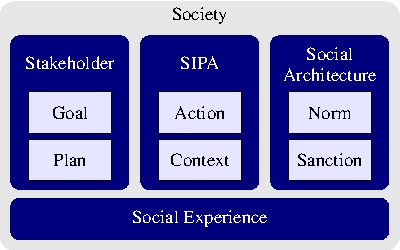
\includegraphics[width=0.6\columnwidth]{poros-nsa-v18-figure0}
\caption[A society of SIPAs and stakeholders]{A society of SIPAs and stakeholders.}
\label{fig:Poros-model} 
\end{figure}

\fbf{The stakeholders} are users, \emph{primary} or \emph{secondary}, depending on the context (defined later).
The \emph{primary} stakeholder of a SIPA is the user who directly interacts with it, and on whose behalf the SIPA acts and interacts.
A \emph{secondary} stakeholder is the user who may not directly interact with the SIPA, but is affected by the SIPA's actions \citep{Ajmeri-AAMAS17-Arnor}. 
Each stakeholder has goals and plans.

\begin{itemize}[nosep]
  \item A \emph{goal} of a stakeholder describes a state the stakeholder would prefer; a stakeholder may have multiple goals.
  \item A \emph{plan} of a stakeholder is a set of actions that can bring about one or more goals.
\end{itemize}

\fbf{The social architecture} of a society captures its structure; it comprises social norms and the sanctions that promote or ensure compliance with norms.

\begin{itemize}[nosep]
  \item A \emph{norm} is a tuple of $\langle$subject, object, antecedent, consequent, context$\rangle$ \citep{Singh-2013-Norms}. 
    Norms characterize the social architecture that promotes prosocial behavior. 
  \item A \emph{deviation} from a norm occurs when a stakeholder, or \emph{deviant}, performs an action that does not comply with it.
  \item A \emph{sanction} is a set of actions a stakeholder may take toward a deviant on observing a deviation. A sanction may be positive or negative \citep{Nardin-KER16-Classifying}.
\end{itemize}

\fbf{A SIPA} acts and interacts on behalf of a stakeholder and
is aware of the social architecture of the society.

\begin{itemize}[nosep]
  \item An \emph{action} is a step a SIPA takes to execute its
    stakeholder's plan, thereby bringing about the corresponding goal.
    An action may satisfy or violate a norm. SIPAs in a society can
    observe each other's actions. 

  \item A \emph{context} captures the circumstances under which a SIPA acts \citep{Dey-2001-Context}. In our approach, the context is social and incorporates whether a norm is satisfied or violated. 
     Context includes social relationships between stakeholders and spatiotemporal parameters relevant to describing interactions between a SIPA and its stakeholders. We adopt Murukannaiah and Singh's \shortcite{IC-Platys-12} notion of \fsl{place} as a location such as home, library, meeting, or party understood in conceptual terms. Parameters describing a place may include physical conditions (e.g., noise level), expected activities (e.g., reading a book), social interactions (e.g., having a discussion), and temporal information (e.g., during office hours on a weekday). 

\end{itemize}

\fbf{The social experience} a SIPA delivers reflects the extent to which the SIPA promotes its primary and secondary stakeholders' goals. It relates to how a SIPA's stakeholders perceive a norm deviation, and the sanctions they apply. Our objective is to promote each SIPA to act toward maximizing the overall social experience, despite competing interests. 

We define social experience ($E$) as the weighted aggregation of payoffs perceived by a SIPA's stakeholders for each action executed by the SIPA. That is, for each potential action, a SIPA determines the payoffs for its primary and secondary stakeholders, and computes an aggregation as a weighted sum of the payoffs.
%
A SIPA's aggregation method reflects its primary user's preferences and privacy attitudes. For instance, a pragmatic user's SIPA may aggregate payoffs by giving equal weight to all stakeholders, whereas a selfish user's SIPA may give a smaller weight to secondary stakeholders.

% Was \paragraph
\subsubsection{\frameworkB Explained with an Example SIPA} 
%
We now describe \frameworkB, a framework to build SIPAs, using \ringer, an example SIPA who answers or ignores phone calls on behalf of its primary stakeholder by ringing the phone or keeping it silent. \ringer is a privacy-enhancing technology that acts on behalf of its primary stakeholder; it determines when to allow intrusions, and when to risk being overheard in a phone call (and thus when to intrude on others' solitude).

\ringer's primary stakeholder is the \fsl{callee} with privacy goals of \fsl{being reachable by phone}, \fsl{to work uninterrupted}, and \fsl{to not disturb neighbors}. \ringer's secondary stakeholders are (1) a \fsl{caller} with the goal \fsl{to reach the callee}; and (2) a \fsl{neighbor} with a privacy goal \fsl{to not be disturbed}. \ringer observes other SIPAs' actions and potentially sanctions them based on their actions and the context as revealed by them.

Each SIPA in \frameworkB maintains a history of interactions and the associated experience. The actual experience is determined after each interaction based on the revealed context and any resulting sanctions. The history helps a SIPA determine the action that would maximize its stakeholder's predicted social experience. 

We define a SIPA's history ($H$) as a set of tuples $h_i = \langle c_i, g, p, N, s_i \rangle$, each of which describes an interaction $i$, including context $c_i$ describing the circumstances in which goal $g$ is brought about via plan $p$ under a set of applicable norms $N$, and all resulting sanctions $\{s_i\}$. 
%
For \ringer, $c_i$ includes the places where the stakeholders are, their social relationships, and urgency of the incoming call.

Each SIPA maintains its history locally, and scans it when selecting a plan. In a conflict situation, SIPAs look up their history to predict social experience and decide which norms or goals to prefer over which others in a given context; thus infer contextually-relevant norms.

A SIPA's behaviors include acting on behalf of its stakeholder, deciding whether to reveal its context, reasoning about the contexts revealed by others, and issuing sanctions to others. It does so based on knowledge of its context, its stakeholder's goals, associated plan, and applicable norms.

\begin{itemize}
    \item \fsl{Plan selection.} A SIPA selects a plan (and its associated actions) that would achieve its primary stakeholder's goals. In the \ringer example, it selects to ring or keep silent for an incoming phone call. If more than one plan are available, from the history (if available) it identifies the one that maximizes the social experience, or chooses a random plan from the applicable plans with a small probability $\alpha$.  
    
    \item \fsl{Revealing context.} When a SIPA chooses and executes a plan, it might deviate from some applicable norms. It decides which norms to prefer in the current context and whether to reveal unobserved context to other SIPAs. For instance, if \ringer decides to prefer the \fsl{family norm}---\fsl{always answer calls from family} over the \fsl{meeting norm}---\fsl{never answer calls during meetings} by ringing during a meeting for an urgent phone call from a sick family member, it reveals the unobserved context, i.e., urgency of the call and the caller's sickness to other meeting attendees. Ideally, a SIPA should selectively reveal context to others according to its stakeholder's goals and privacy attitude. 
    
    \item \fsl{Sanctions.} A SIPA observes other SIPAs' actions, and sanctions them when its stakeholder is affected by their actions. On receiving the context revealed by a deviating SIPA, the SIPA of an affected stakeholder evaluates whether the observed action would be norm compliant in the revealed context. In the \ringer example, \fsl{neighbors'} and \fsl{caller's} SIPAs decide whether they would ring for an urgent phone call from a sick family member during a meeting and accordingly sanction the \fsl{callee's} SIPA. 
\end{itemize}

The complete interaction, including the selected plan and executed actions, observed and revealed context, applicable norms, and sanctions, is recorded in SIPAs history. 
As SIPAs interact by acting and evaluating actions for norm compliance from interaction history, they understand the boundaries of applicable norms in different contexts, and thus promote emergence of robust social norms. 


\section{Simulation Model}
\label{sec:Poros-simulation-model}

We evaluate \frameworkB via a simulated 
\emph{ringer environment} built using MASON \citep{Luke-2005-Mason}.

\subsection{The Ringer Environment}
The ringer environment contains shared places (home, party, meeting, library, and emergency room).
Corresponding to each place, we define social circles such as family, friends, and coworkers. Each agent belongs to a family circle, a friend circle, and a coworker circle. Agents who do not share any of these circles are considered strangers. We define the social network or place network topology in a way such that there is only one type of relationship, i.e., family, friends, coworkers, or strangers, between any pair of agents. 
In the ringer environment, there are (1) several homes, each corresponding to a family circle, (2) several parties, corresponding to multiple friend circles, and (3) multiple meetings, corresponding to multiple colleague circles. There is one library and one emergency room (ER). The numbers of homes, parties, and meetings follow the network setups specified in Table~\ref{tab:network-types}.

%\paragraph{Moving between places}
In the simulation, agents stay at each place for a random number of steps (averaging 60 steps) and then move. If an agent enters home, party, or meeting, it is more likely to enter the place that is associated with its own social circle than entering a place with strangers. For example, if an agent chooses to enter home, it is likelier to enter its own family's home than to enter a stranger's home. Therefore, when it is at home, an agent is usually surrounded by its family members with only a few strangers. 

%\paragraph{Actions}
The agents in the ringer environment perform the following actions depending upon their roles:
\begin{itemize}
\item A caller initiates an urgent or a casual phone call.
\item A callee answers or ignores a phone call.
\item A callee shares context for answering or ignoring a call.
\item A caller and neighbors respectively reason about context.
\item A caller and neighbors respectively sanction a callee for answering or ignoring a phone call.
\end{itemize}

%\paragraph{Norms}
Each place and each circle has predefined norms, as defined in Table~\ref{tab:norms-place}. For example, emergency room (ER) is conceptualized as a place where the default norm is to always answer calls, whereas the norm in a library is to ignore calls. Norms could conflict. For example, the norm to \fsl{answer an urgent phone call from a family member} conflicts with \fsl{ignore during a meeting}. We let the agents figure out contextually relevant norms in case of conflict. 

\begin{table}[!tb]
\centering

\caption[Norms for answering calls]{Norms for answering calls based on (left) place and (right) caller's social circle and casual or urgent call types.}
\label{tab:norms-place}

\begin{tabular}{@{} c @{~~~~} c @{}}

\begin{tabular}{@{~~}l@{~} c@{}}
\multicolumn{2}{c}{\fbf{By place}}\\
\toprule
Place & Response\\\midrule
Emergency (ER) &Answer\\
Home (H) & Answer \\
Library (L) &Ignore\\
Meeting (M) &Ignore\\
Party (P) &Answer\\
\bottomrule
\end{tabular}
&
\begin{tabular}{@{}l @{~} c@{~} c@{~~}}
\multicolumn{3}{c}{\fbf{By circle and call type}}\\
\toprule
Circle & Casual & Urgent\\
\midrule
Coworker&Answer&Answer\\
Family&Answer&Answer\\
Friend&Answer&Answer\\
Stranger&Ignore&Answer\\
\bottomrule
\\
\end{tabular}
\end{tabular}
\end{table}

%\paragraph{Payoffs}
For each phone call, based on the callee's response of answering or ignoring, the caller, callee, and neighbors perceive a fixed payoff, as shown in Tables~\ref{tab:payoff-callee}--\ref{tab:payoff-neighbor}. 


\begin{table}[!tb]
\centering

\caption[Payoff for callee]{Payoff for callee for casual or urgent call types.}
\label{tab:payoff-callee}


\begin{tabular}{@{}lcrr@{}}
\toprule
Caller's Relationship & Callee's Response & Casual & Urgent\\\midrule
\multirow{2}{2.8cm}{Family, Friend, or Coworker}&Answer&0.50&1.00\\
&Ignore&0.00&--0.50\\\midrule
\multirow{2}{2.8cm}{Stranger}&Answer&0.00&0.50\\
&Ignore&0.25&--0.25\\
\bottomrule
\end{tabular}


\end{table}

\begin{table}[!tb]
\centering

\caption[Payoff for caller]{Payoff for caller for casual or urgent call types.}
\label{tab:payoff-caller}

\begin{tabular}{@{}crr@{}}
\toprule
Callee's Response & Casual & Urgent\\\midrule
Answer&0.50&1.00\\
Ignore&--0.50&--1.00\\\bottomrule
\end{tabular}

\end{table}

\begin{table}[!tb]
\centering

\caption[Payoff for neighbors]{Payoff for neighbors by place (ER, H, L, M, P).} 
\label{tab:payoff-neighbor}

\begin{tabular}{@{}crrrrr@{}}
\toprule

% Callee's Response & ER & H & L & M & P \\\midrule
Callee's Response & Emergency & Home & Library & Meeting & Party \\\midrule
Answer & 1.00 & 0.67 & --1.00 & --1.00 & --0.33\\
Ignore & --1.00 & --0.33 & 1.00 & 1.00 & 0.67\\\bottomrule

\end{tabular}

\end{table}

\subsection{Agent Types}
\label{sec:agent-types}

To evaluate effectiveness of \frameworkB, we define two baseline agent types---\emph{Fixed} and \emph{Sanctioning}, other than \frameworkB agents.

\emph{Fixed agents} act according to the fixed set of norms listed in
Table~\ref{tab:norms-place}. If the norms conflict, the agents toss a
fair coin to choose between alternative actions. If Fixed agents
perceive an action as a deviation, they sanction the deviant.

\emph{Sanctioning agents} infer social norms from sanctions
\citep{Andrighetto-2013-PunishVoice}. These
agents start with the same strategy as Fixed agents. They continue to record 
the interaction history. Once they have gained enough number of records in their
history of sanctions, they decide their subsequent actions based on
history. In our simulation, this number is empirically selected so that an
agent visits each scenario at least once. As callees,
when norms conflict, they select the action that provides a higher payoff, computed according to Tables~\ref{tab:payoff-callee}--\ref{tab:payoff-neighbor}. As callers
and neighbors, these agents sanction callees as per fixed norms listed
in Table~\ref{tab:norms-place}.

\emph{\frameworkB agents} infer social norms by revealing and reasoning
about context. They start with the same strategy as Fixed
agents following norms listed in Table~\ref{tab:norms-place}. As
callees, they reveal context, i.e., reveal the caller's relationship and
the call's urgency to their neighbors, and reveal their place and 
neighbors' relationships to the caller. As neighbors or callers, they
understand the callee's revealed context and decide what action they would
have performed were they in that context, and sanction
accordingly. \frameworkB agents use Table~\ref{tab:payoff-neighbor-reason}'s payoffs.

We employ a linear regression model over interaction history to
choose actions based on sanctions by stakeholders.


\begin{table}[!tb]
\centering

\caption[Payoffs based on reasoning about the shared context]{Payoff for a neighbor based on how callee acts and what the neighbor expects in the context revealed by callee.}

\begin{tabular}{@{}c @{~~} c@{~~} r@{~~} r@{~~} r@{~~} r@{~~} r@{}}
\toprule
% Callee Action&Neighbor Expects
%  & ER & H & L & M & P\\\midrule

Callee Action&Neighbor Expects
 & Emergency & Home & Library & Meeting & Party\\\midrule

Answer&Answer & 1.00 & 0.67 & 1.00 & 1.00 & 0.67 \\
Answer&Ignore & --1.00 & --0.33 & --1.00 & --1.00 & --0.33 \\
Ignore&Answer & --1.00 & --0.33 & --1.00 & --1.00 & --0.33 \\
Ignore&Ignore & 1.00 & 0.67 & 1.00 & 1.00 & 0.67\\\bottomrule

\end{tabular}

\label{tab:payoff-neighbor-reason}

\end{table}

\section{Experiments and Results}
\label{sec:Poros-experiments}

We evaluate our research questions via multiple experiments 
on the ringer environment in which we
simulate \np{1000} or 250 Fixed, Sanctioning, and \frameworkB agents in pragmatic, considerate, and selfish agent societies. The agents in societies use different schemes to aggregate payoffs. We run each
simulation for \np{3000} steps and compute the following metrics.

\begin{description}
\item[Social cohesion] measures the proportion of agents that perceive actions
as norm compliant. Higher the social cohesion, lower is the number of negative sanctions.

\item[Social experience] measures the goal satisfaction delivered by an agent, 
computed by aggregating payoffs for all stakeholders according to
the payoff Tables~\ref{tab:payoff-callee}, \ref{tab:payoff-caller},
\ref{tab:payoff-neighbor}, and \ref{tab:payoff-neighbor-reason}.

\end{description}

To answer \fsl{Q$_1$} on norms, we consider the following hypotheses pertaining to specified agent types. For brevity, we omit 
the corresponding null hypotheses indicating no gain. We test significance via the two-tailed paired $t$-test. 
\begin{description}
\item[H$_1$] \frameworkB yields greater \fsl{social cohesion} than Fixed.
\item[H$_2$] \frameworkB yields greater \fsl{social cohesion} than Sanctioning.
\end{description}

To answer \fsl{Q$_2$} on goals, we consider these hypotheses:
\begin{description}
\item[H$_3$] \frameworkB yields greater \fsl{social experience} than Fixed.
\item[H$_4$] \frameworkB yields greater \fsl{social experience} than Sanctioning.
\end{description}



\subsection{Experiments with Pragmatic Agent Society and Varying Network Types}
\label{sec:experiment1}

We simulate Fixed, Sanctioning, and \frameworkB agents on four network types---large or small network with dense or sparse connectivity---as Table~\ref{tab:network-types} describes. The society in this experiment is pragmatic in that the agents perceive social experience as the average payoff (equally weighted) for all stakeholders in an interaction.
%
We summarize our results next.


\begin{table}[!tb]
\centering

\caption[Characteristics of network types studied]{Characteristics of network types studied.}
\label{tab:network-types}

\begin{tabular}{@{}crrrr@{}}
\toprule
\multirow{2}{*}{\fbf{Network Type}} & \multirow{2}{*}{\fbf{Agents}} & \multicolumn{3}{c}{\fbf{Circles}}\\
\cmidrule{3-5}
&&Family&Coworker&Friend\\
\midrule
Large Dense & \np{1000} & 20 & 20 & 20\\
Large Sparse& \np{1000} & 100 & 100 & 100\\
Small Dense & 250 & 5 & 5 & 5\\
Small Sparse& 250 & 25 & 25 & 25\\
\bottomrule
\end{tabular}

\end{table}

\begin{description} 
\item[Fixed agents.] 
The average social experience was found to be
between 0.53 and 0.56, and the social cohesion to be about 52\% for the
four network types.

\item[Sanctioning agents.] 
As expected, at around step \np{1000} we see Sanctioning agents offer a rise in
social experience over Fixed agents. The rise
is gradual as the agents start to infer from history. For the first \np{1000} steps, the
average social experience is the same as Fixed agents. It later
stabilizes between 1.11 and 1.21 for all four networks. The social cohesion
values were between 61.2\% and 63.7\%.

\item[\frameworkB agents.] 
At around step \np{1000}, as agents acquire confidence,
we see a significant increase in social experience offered by \frameworkB
agents. It stabilizes between 2.14 and 2.19 for the different networks.
Social cohesion was found be significantly higher between 82.0\% and 83.2\%.
For the first \np{1000} steps, \frameworkB agents yield the same average social
experience as Fixed and Sanctioning agents. 
\end{description}

Social cohesion and experience offered by \frameworkB agents are 
significantly greater than those offered by Fixed and Sanctioning agents;
thus the null hypotheses corresponding to H$_1$, H$_2$, H$_3$,
and H$_4$ are rejected. Figure~\ref{fig:experiment1-results} shows
the social experience plots indicating the results are consistent across
the four network types. Table~\ref{tab:experiment1-results} summarizes
the findings of the experiment with pragmatic agents.
It shows stabilized values for social experience and social cohesion, and p-values from the two-tailed paired $t$-tests.

\begin{figure}[!tb]
    \centering

\caption[Social experience plots for different networks]{Social experience yielded by Poros, Sanctioning, and Fixed agents (per phone call for a window size of $200$ steps) in pragmatic agent societies of different network sizes and densities.
}
    \label{fig:experiment1-results}

    
\begin{tabular}{@{}cc@{}}

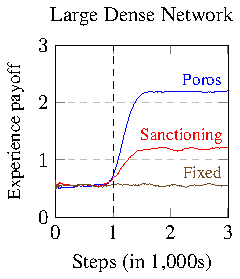
\includegraphics[width=0.40\columnwidth]{poros-nsa-v18-figure2.pdf}
&
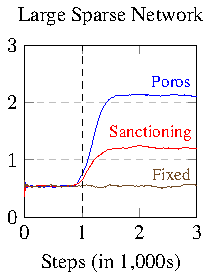
\includegraphics[width=0.35\columnwidth]{poros-nsa-v18-figure3.pdf}
\\
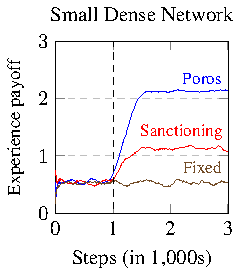
\includegraphics[width=0.40\columnwidth]{poros-nsa-v18-figure4.pdf}
&
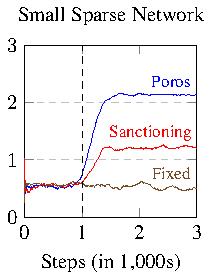
\includegraphics[width=0.35\columnwidth]{poros-nsa-v18-figure5.pdf}
\end{tabular}

\end{figure}


\begin{table}[!tb]
\centering

\caption[Effectiveness of \frameworkB in a pragmatic society]{Effectiveness of \frameworkB in a pragmatic society.}
\label{tab:experiment1-results}

\begin{tabular}{@{~~~} c@{~~~~} l@{~~~} r@{~~~} r@{~~~} r@{~~~}}

\toprule
& Agent Type & Experience & Cohesion & $p$\\
\midrule
\multirow{3}{*}{\rotatebox[origin=c]{90}{\parbox[c]{33pt}{\centering Large Dense}}}
&Fixed & 0.56 & 52.7\% & $<$ 0.01\\
%
&Sanctioning & 1.21 & 63.5\%  & $<$ 0.01\\
%
&\frameworkB & 2.19 & 83.2\%  & -- \\
\midrule
\multirow{3}{*}{\rotatebox[origin=c]{90}{\parbox[c]{33pt}{\centering Large Sparse}}}
&Fixed & 0.55   & 52.5\%  & $<$ 0.01 \\
&Sanctioning & 1.21   & 63.5\%  & $<$ 0.01 \\
&\frameworkB & 2.19  & 83.2\%  & --\\
\midrule
\multirow{3}{*}{\rotatebox[origin=c]{90}{\parbox[c]{33pt}{\centering Small Dense}}}
&Fixed & 0.53   & 52.1\%  & $<$ 0.01 \\
&Sanctioning & 1.11   & 61.2\%  & $<$ 0.01 \\
&\frameworkB & 2.14  & 82.0\%  & --\\
\midrule
\multirow{3}{*}{\rotatebox[origin=c]{90}{\parbox[c]{33pt}{\centering Small Sparse}}}
&Fixed & 0.54  & 52.5\%  & $<$ 0.01 \\
&Sanctioning & 1.22   & 63.7\%  & $<$ 0.01 \\
&\frameworkB & 2.14  & 82.1\% & --\\
\bottomrule
\addlinespace
\end{tabular}

\end{table}

\subsection{Experiment with Considerate Agent Society} 
We experiment with a considerate agent society where agents give a larger weight to their neighbors' payoffs 
than to their own payoffs when computing social experience and deciding the actions to perform when norms
conflict. These agents continue to sanction based on their history.

%\paragraph{Results} 
Figure~\ref{fig:experiment2-considerate-selfish}
shows the social experience for considerate Sanctioning and \frameworkB
agents in a Small-Dense network. The average social experience drops for
Sanctioning and \frameworkB agents after they have gained enough
confidence. We attribute this decline to the fact that these agents
value the neighbors' experience more than their own, and thus
ignore calls they should have answered. \frameworkB agents
offer higher social cohesion and experience than Sanctioning agents because the
secondary stakeholders give smaller negative sanctions when they reason about
context. The results for the other three network types are similar.
Table~\ref{tab:experiment2-results} summarizes these results.

\begin{table}[!tb]
\centering

\caption[Effectiveness of \frameworkB in considerate and selfish societies]{Effectiveness of \frameworkB in considerate and selfish societies.}
\label{tab:experiment2-results}

\begin{tabular}{@{~~~} c@{~~~~} l@{~~~} r@{~~~} r@{~~~} r@{~~~}}

\toprule
& Agent Type & Experience & Cohesion & $p$\\
\midrule
\multirow{2}{*}{\rotatebox[origin=c]{90}{\parbox[c]{22pt}{\centering\small Consi-derate}}}
&Sanctioning & --0.33   & 41.3\%  & $<$ 0.01 \\
&\frameworkB & --0.14  & 48.4\% & --\\

\midrule
\multirow{2}{*}{\rotatebox[origin=c]{90}{\parbox[c]{22pt}{\centering\small Selfish}}}
&Sanctioning & 1.22   & 63.5\%  & $<$ 0.01 \\
&\frameworkB & 2.13  & 82.0\% & --\\

\bottomrule
\addlinespace

\end{tabular}

\end{table}

\subsection{Experiment with Selfish Agent Society} 
In a selfish agent society, agents give a very large weight to their own payoffs 
when computing social experience. Agents here may not always negatively sanction 
others who disturb them. As in other societies, agents in a selfish society sanction a deviant based on their history.

%\paragraph{Results}
Figure~\ref{fig:experiment2-considerate-selfish}
shows the social experience plot for selfish Sanctioning and \frameworkB agents
in a Small-Dense network. The plots resemble those in the
experiment with pragmatic agents, but with slightly lower stabilized
values. Here, agents tend to answer all calls, which benefits both
caller and callee most of the time. We observe similar results for the
other three networks. Table~\ref{tab:experiment2-results} summarizes
these results. 

\begin{figure}[!tb]
\centering
    
\begin{tabular}{@{}cc@{}}

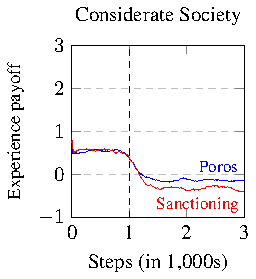
\includegraphics[width=0.40\columnwidth]{poros-nsa-v18-figure6.pdf}
&
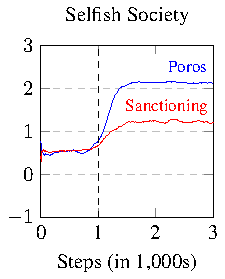
\includegraphics[width=0.35\columnwidth]{poros-nsa-v18-figure7.pdf}
\end{tabular}
\caption[Social experience plots for considerate and selfish agents]{Social experience (averaged over a window size of 200 steps)
yielded by Poros and Sanctioning agents in considerate and selfish agent societies simulated in a Small-Dense network.}
\label{fig:experiment2-considerate-selfish}

\end{figure}

\subsection{Threats to Validity}

%\paragraph{Threats Mitigated}
We identified and mitigated two threats. The first concerns
a differences in how users perceive experience.
In reality, not all users perceive social experience the same way, and thus aggregating with only one scheme introduces the threat of difference in perceiving social experience. To mitigate this threat, we conduct experiments with three agent societies with different experience aggregation schemes.
%
The second threat concerns scalability. Since we simulate agent actions and interactions, a threat is whether our results scale to a large number of agents. To mitigate this threat, we evaluate \frameworkB considering varying network sizes and types. 

%\paragraph{Threats Remaining}
However, some threats remain. In particular, first, our results are based on simulation. Testing a SIPA's adaptability with end-users across contexts is challenging, as is reliably eliciting user attitudes and preferences. 

Second, \frameworkB agents always reveal context, which may pose a privacy threat. Ideally SIPAs should reveal context selectively. We leave this reasoning for future studies. 

\section{Conclusion and Future Directions}
\label{sec:Poros-discussion}

In \frameworkB, SIPAs reveal and reason about context to understand the boundary of applicable norms and infer contextually relevant social norms. 
We find that \frameworkB agents deliver significantly higher (1) social cohesion and (2) social experience than other agents. These findings are stable under changes to network size and characteristics of agents.

Being sensitive to norms, \frameworkB SIPAs can naturally address challenges in engineering software tools for privacy.  A SIPA would need data about its user's sharing preferences, privacy attitudes, and values and ethics \citep{Ajmeri-IC18-Ethical} to make effective recommendations. A SIPA can learn its user's preferences and attitudes, but it would be helpful to bootstrap a SIPA via crowdsourced data about diverse user classes \citep{TOCHI-17:Multiuser,IC-17:SoSharP}. To better support privacy-respecting SIPAs, \frameworkB could incorporate characteristics suggested by Such \shortcite{Such-IJCAI17-Privacy} and adopt argumentation as in K{\"o}kciyan and Yolum's \shortcite{Kokciyan-IJCAI17-Privacy} work when deciding the subset of context to reveal.

Other future directions are incorporating affect in relation to norms
\citep{Ferreira-AAAI13-GroupRelations} 
and supporting white lies to promote privacy (and social cohesion). For example, Bob may say his son is in hospital, instead of drug rehab. It would be instructive to study how such deception modulates 
effects on norms and goals.